\chapter{Attack Scenarios}\label{attacks}

This section covers some of the possible attack scenarios and how the Tangle can still maintain consensus among honest users.

\section{Double Spend}
A double spend situation occurs when a user tries to exceed his account balance by issuing two or more conflicting transactions. Figure \ref{fig:double-spend} illustrates such a scenario. A box represents a transaction. The dashed box inside represents the current state in the graph but is not part of an actual transaction. In this simulation, Alice owns only 15 IOTA but issues two transactions with 10 IOTA each. Bob cannot approve both of Alice's transactions as they result in a negative account balance.

\begin{figure}[H]
    \centering
    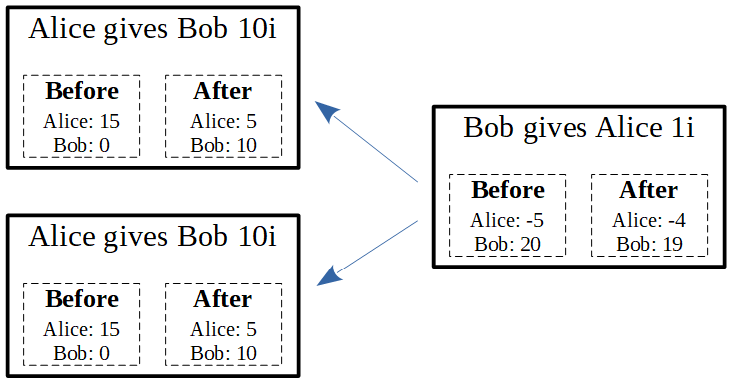
\includegraphics[width=8cm]{images/double-spend.png}
    \caption{Double Spend Attack \cite{the-tangle-part-5}}
    \label{fig:double-spend}
\end{figure}

The solution to this problematic situation is the weighted random walk discussed in Section \ref{tip-selection}. One of the two transactions will become heavier and the lighter one will be abandoned. This implies that a confirmed transaction cannot be considered as valid as soon as it has been approved for the first time. 

Confirmation confidence is introduced in Section \ref{transaction-validation} and provides a measurement of what percentage the network has directly or indirectly approved a transaction. 


\section{Large Weight Attack}
The large weight attack has the same intent as the double spend but actively tries to invalidate a transaction with high confirmation confidence. This can be achieved by a malicious user as follows.

\begin{enumerate}
    \item A transaction is created and broadcasted that is intended to revert.
    \item The malicious user waits until the receiver believes the transaction has a high enough confirmation rate. The merchant ships the product/service.
    \item The attacker uses its computational power and issues a double-spending transaction with a large weight followed by many more transactions. This transaction does not approve the first transaction and thus they compete with each other for finality.
    \item The bad actor hopes that the dishonest subtangle gains more cumulative weight than the honest subtangle.
\end{enumerate}

\begin{figure}[H]
    \centering
    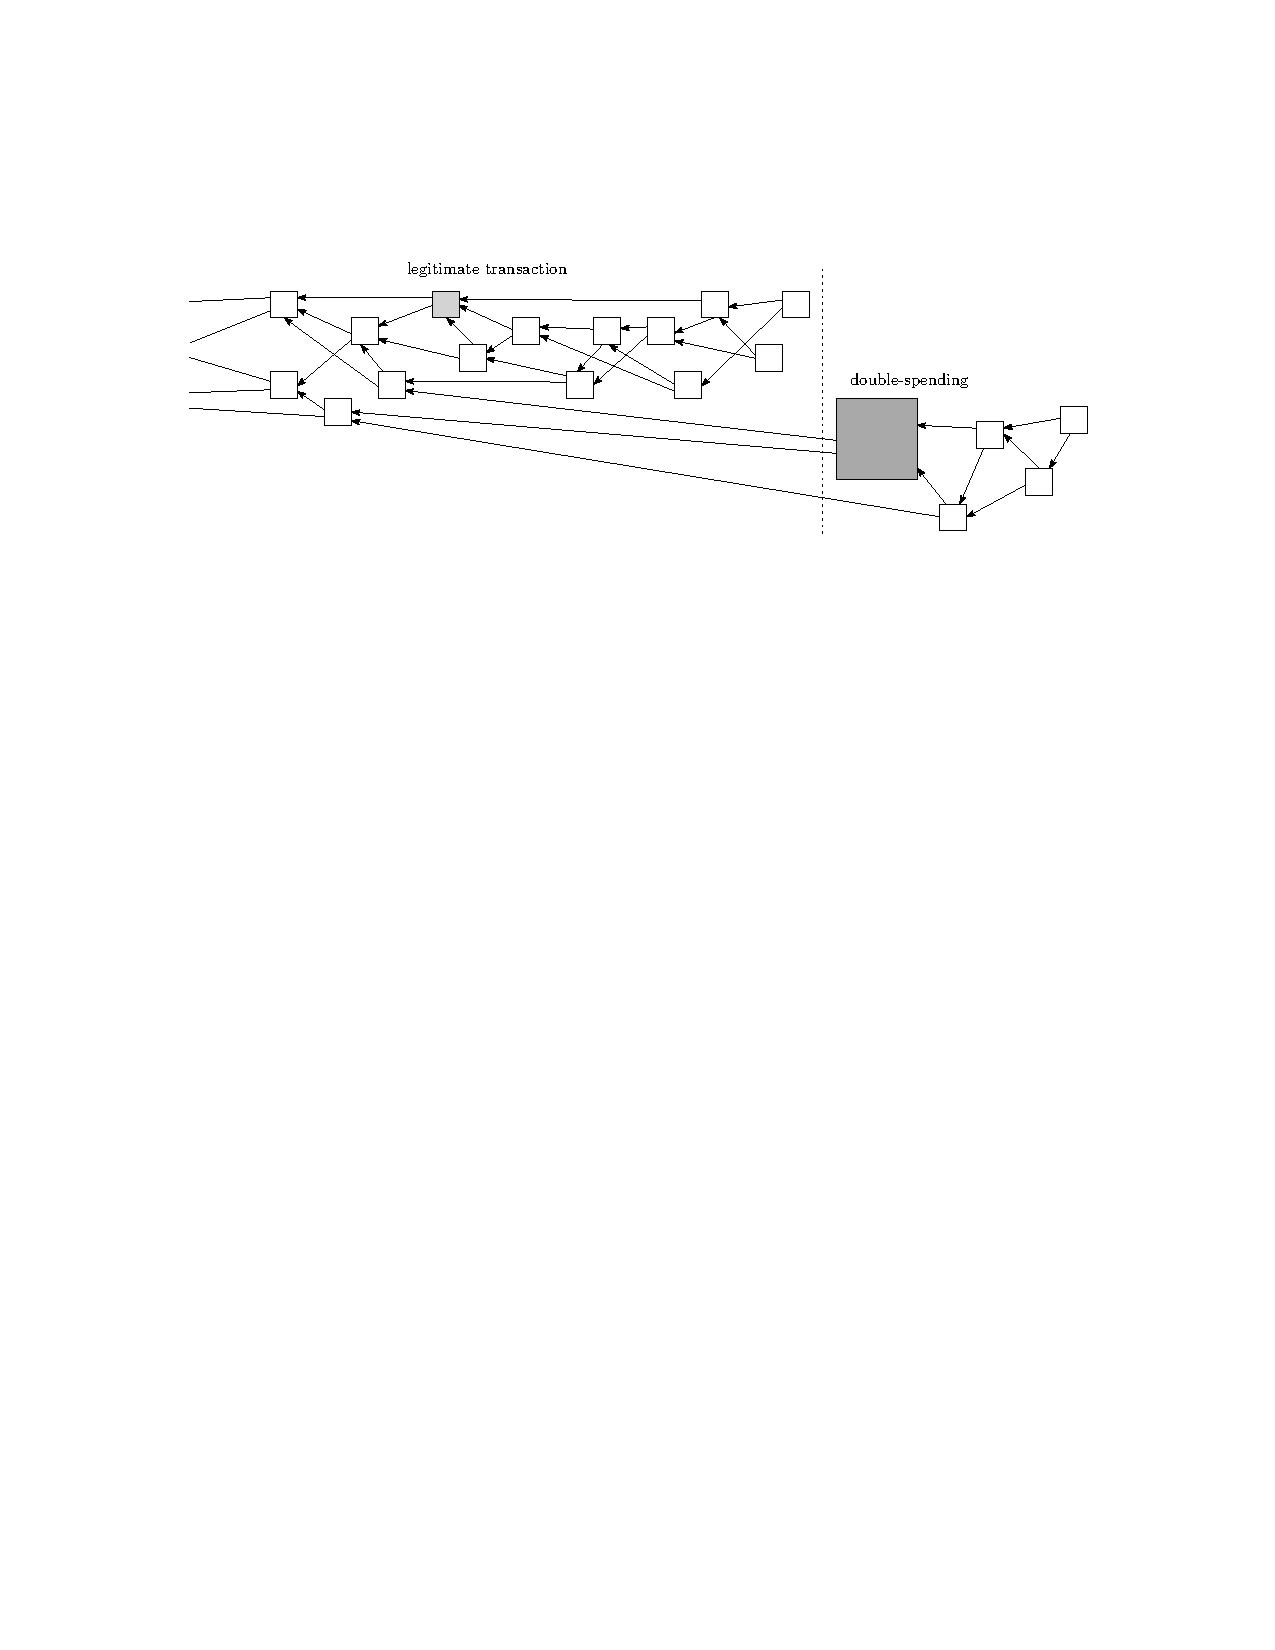
\includegraphics[width=12cm]{images/large-weight-attack.pdf}
    \caption{Large Weight Attack \cite{the-tangle}}
    \label{fig:large-weight-attack}
\end{figure}

This attack can only be carried out if the attacker has more computing power than all the nodes that actively issue new transactions. In a well-established network with many nodes issuing transactions, this is less of an issue. In the early stages, however, there are not enough transactions passing through the network in order to be safe from such an attack. Due to this reason, the IOTA foundation has put a coordinator in place which is discussed in more detail in Section ?.

\section{Parasite Chain Attack}
The parasite chain attack also tries to convince the network to abandon a previously confirmed transaction by biasing the tip selection algorithm.The attack works as follows:
\begin{enumerate}
    \item The attacker creates a transaction branching off from the main tangle (MT). He does not broadcast this transaction. This transaction is the red dot furthest to left in Figure \ref{fig:parasite-chain}.
    \item Instead, he keeps adding new transactions to this local chain called parasite chain (PC).
    \item He makes sure, that he references the MT within the PC.
    \item The malicious user creates a transaction on the MT which he hopes to get abandoned by the network when he publishes the parasite chain. This transaction is the red dot furthest to right.
    \item The user waits until the transaction on the MT is considered as validated. During this time he keeps building on the PC but can only reference transactions before the double-spend transaction on the MT.
    \item At this point, the bad actor broadcasts the parasite chain.
    \item Furthermore, he might try to artificially inflate the number of tips on the PC.
\end{enumerate}

The attacker's intention is that new transactions reference the parasite chain such that the MT will be orphaned. 
However, the tips on the parasite chain have a smaller amount of cumulative weight, assumed the attacker has less computational power than the rest of the network. 
Thus, in order to mitigate such an attack, it is important for the MCMC selection algorithm to be biased towards transactions with a high cumulative weight. The tradeoff for setting the bias is discussed in Section \ref{tip-selection}.

\begin{figure}[H]
    \centering
    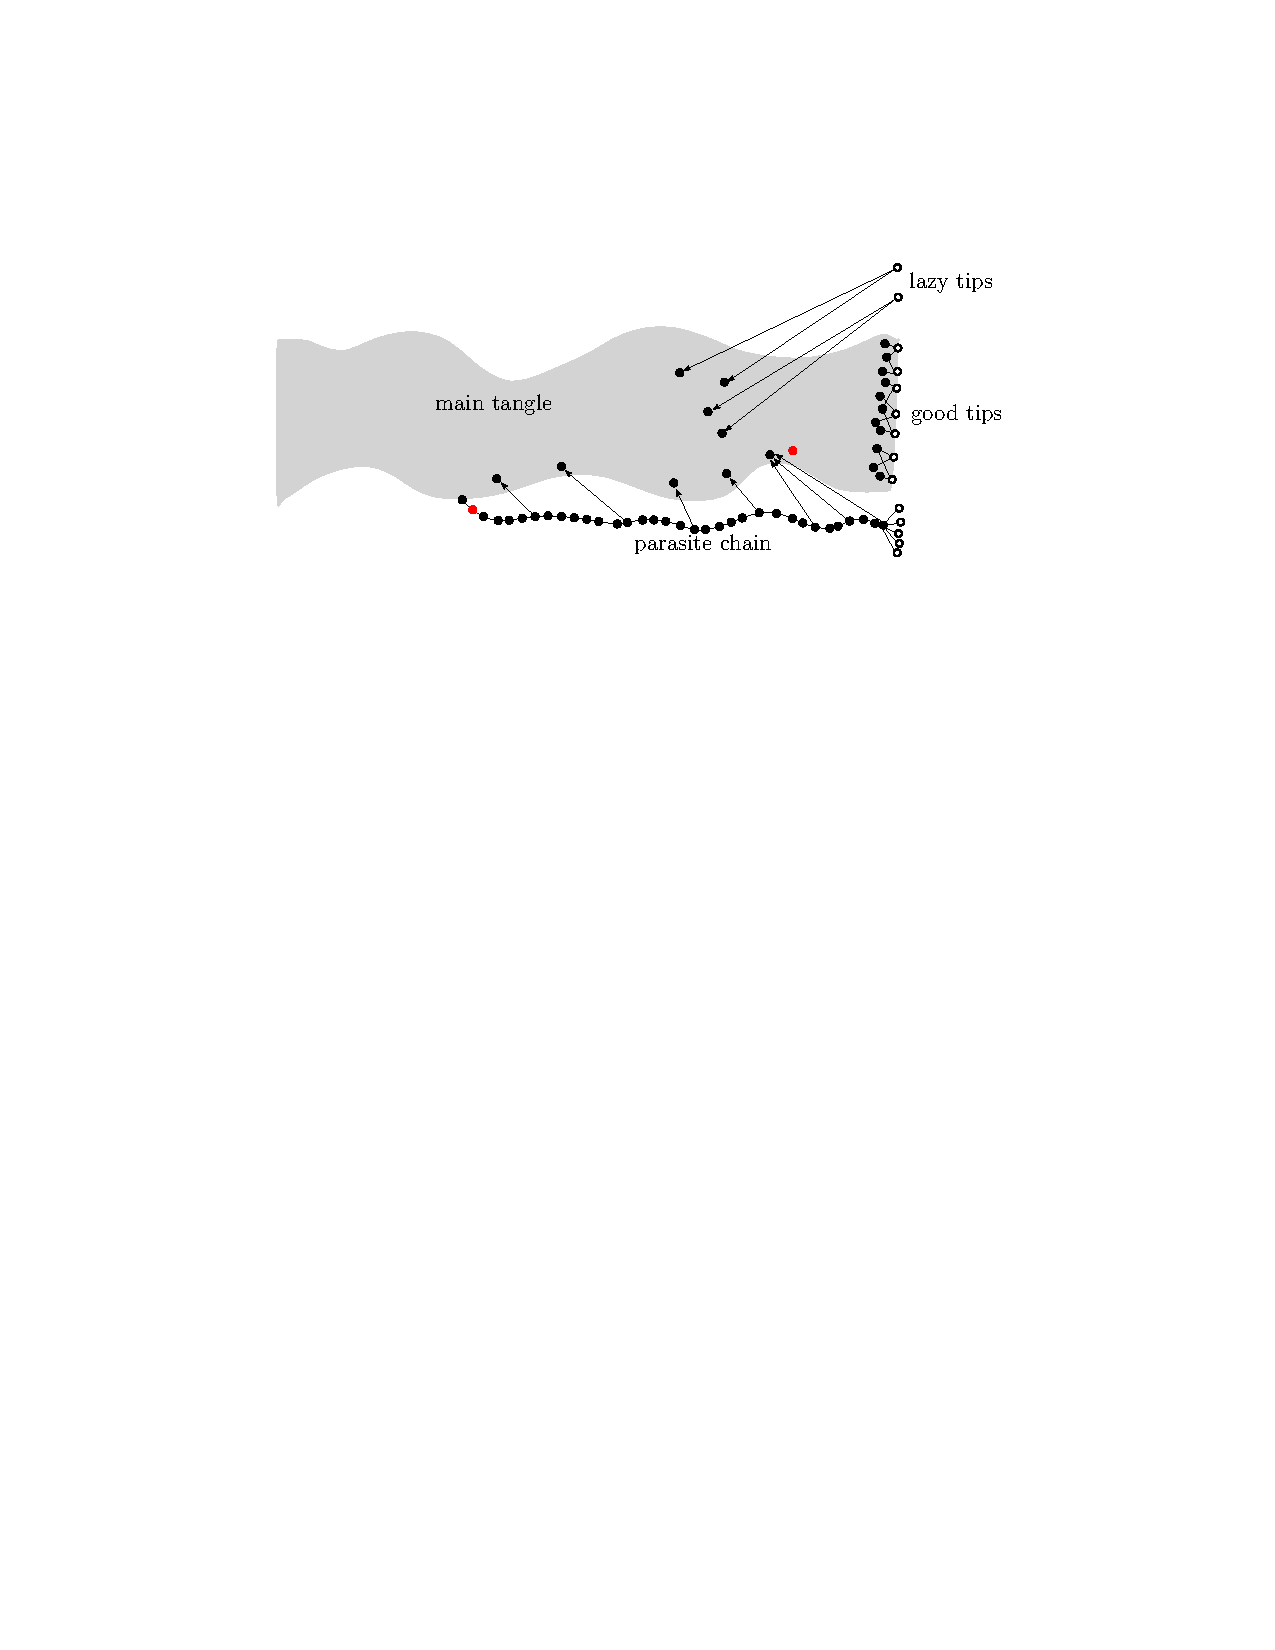
\includegraphics[width=12cm]{images/parasite-chain.pdf}
    \caption{Parasite Chain Attack \cite{the-tangle}}
    \label{fig:parasite-chain}
\end{figure}

